\documentclass[11pt]{article}
\usepackage[letterpaper,margin=1in]{geometry}
\usepackage{color}
\usepackage[dvipdfmx]{graphicx}
\usepackage{amsbsy}
\usepackage{amsmath}
\usepackage{adjustbox}
\usepackage{url}

\newcommand{\argmax}{\mathop{\rm arg~max}\limits}

\begin{document}
\title{Analysis Report on Assignment 1: K-nearest neighbors}
\author{Yoshinari Fujinuma}
\date{}
\maketitle

%\section{What is the relationship between the number of training examples and accuracy?}
\section{The relationship between the number of training examples, $k$, and accuracy}
The following two graph shows the relationship between training examples and accuracy:
\begin{figure}[htb]
  \begin{center}
   \begin{tabular}{c}

    \begin{minipage}{0.5\hsize}
     \begin{center}
     \scalebox{0.33}
      {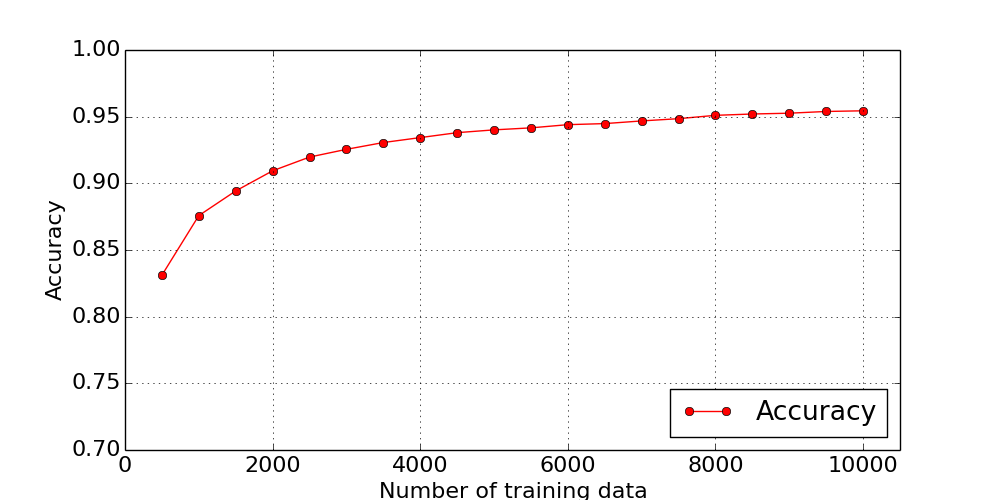
\includegraphics[]{figure_1.png}}
   
      \caption{The relationship between the number of training examples and accuracy. The value of $k$ is fixed to $3$. }
      \label{fig:corpus_size}
     \end{center}
    \end{minipage}

    \begin{minipage}{0.01\hsize}
    \end{minipage}

    \begin{minipage}{0.5\hsize}
     \begin{center}
      \scalebox{0.33}
      {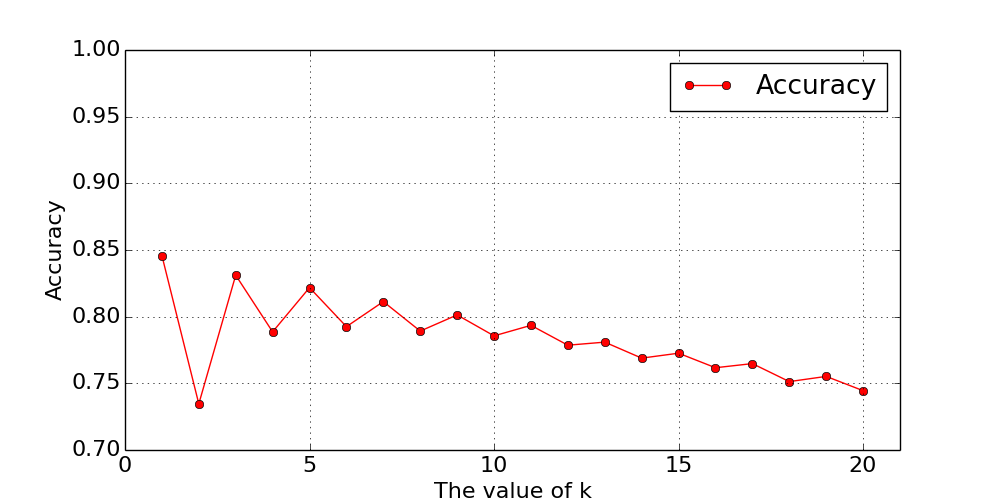
\includegraphics[]{figure_2.png}}
      \caption{\label{k_and_accuracy}The relationship between $k$ and accuracy. The value of the number of training examples is fixed to $500$}
     \end{center}
    \end{minipage}

  \end{tabular}
 \end{center}
\end{figure}

As the number of training examples increases, the higher the accuracy becomes.
The zig-zag observed in Figure \ref{k_and_accuracy} is partly because when the value of $k$ is an even number, then the median returns an answer in decimals (i.e. a label that is not an integer between $0$ and $9$), which causes median tie-breaker to be less reliable. Therefore, the accuracy is generally low when $k$ is an even number.

%\section{What is the relationship between $k$ and accuracy?}
%The following graph shows the relationship between $k$ and accuracy:
%\begin{figure}[htb]
%  %\begin{minipage}{0.5\hsize}
%   \begin{center}
%    \scalebox{0.4}
%     {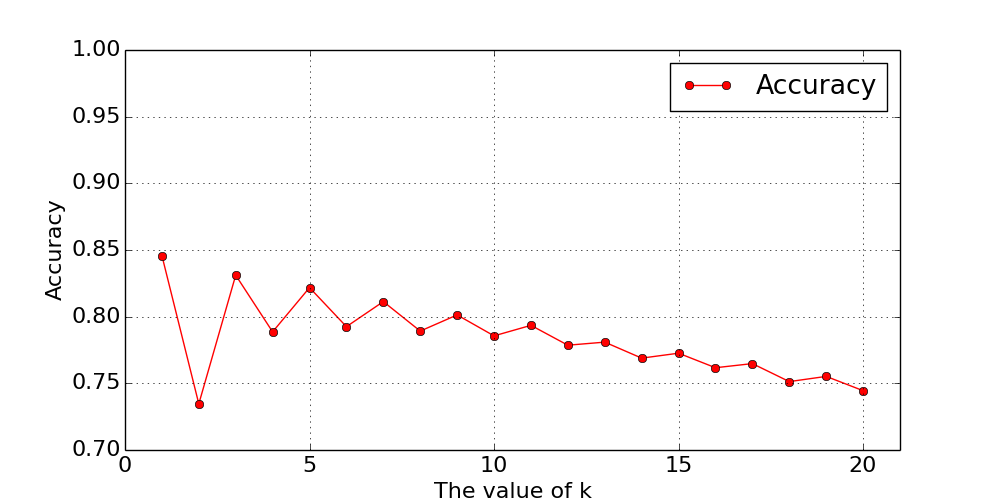
\includegraphics[]{figure_2.png}}
%    \end{center}
%    \caption{The relationship between $k$ and accuracy.}
%    \label{fig:corpus_size}
%  %\end{minipage}
%%\vspace{0.1cm}
%\end{figure}

\section{What numbers get confused with each other most easily?}

By fixing $k = 3$, no matter what the number of training examples is, the classification of $4$ and $9$ easily gets confused. 
Specifically, the test examples that are labeled $4$ are mistakenly classified as $9$.
% few due to the use of the median function to break ties.
% TODO: probably better to have a table here?
Let $limit$ be the number of training examples. 
By further analyzing the possible causes of misclassification, the median tie-breaker between $4$ and $9$ happened the most ($72$ times) when $k = 3$ and $limit = 500$. 
It is possible that the median tie-breaker is causing many misclassifications, because if all of median tie-breaker is causing misclassification, then it covers around half ($72/155$) of the total number of misclassified examples between $4$ and $9$. 
However, we did some further investigation on larger $k$ and larger $limit$. 
When $k = 19$ and $limit = 5000$, the median tie-breaker happened only $8$ times and $62$ test examples of the number $4$ are misclassified as $9$.

In conclusion, the median tie-breaker does not contribute a lot to the most misclassified test examples of $4$ and $9$, and we infer that the misclassification is mainly caused by $4$ and $9$ having a similar structure.

\end{document}

